\documentclass[12pt, a4paper, openany]{book}
\usepackage{../generalStyle}
\usepackage{enumitem}
\usepackage{makecell}

\graphicspath{ {./img/} }
\def\arraystretch{2}
\newcolumntype{Y}{>{\centering\arraybackslash}X} %new tabularx centered X column  

\begin{document}
\title{CheatSheet di Ricerca Operativa e Pianificazione delle Risorse}

\author{
	Fabio Ferrario\\
	\small{\href{https://t.me/fefabo}{@fefabo}}
}
\date{2022/2023}

\maketitle

\tableofcontents

\chapter{Programmazione Lineare}
\section{Il metodo del Simplesso}

\paragraph*{La forma Tabellare}
\begin{center}
	\begin{tabular}{c|c|c|cccc|c}
		\small{V. BASE} & Eq     & Z      & $x_1$    & $x_2$    & ...      & $x_n$    & T. Noto \\
		\hline
		Z               & R$_0$  & 1      & $c_1$    & $c_2$    & ...      & $c_n$    & 0       \\
		$x_1$           & R$_1$  & 0      & $a_{11}$ & $a_{12}$ & ...      & $a_{1n}$ & $b_1$   \\
		\vdots          & \vdots & \vdots & \vdots   & \vdots   & $\ddots$ & \vdots   & \vdots  \\
		$x_m$           & R$_n$  & 0      & $a_{m1}$ & $a_{m2}$ & ...      & $a_{mn}$ & $b_m$   \\
	\end{tabular}
\end{center}

\paragraph{Forma Aumentata} Per portare il problema in forma aumentata:\\
\begin{tabularx}{\textwidth}{|X|lc|c|l|}
	\hline
	\multirow{3}{*}{\textbf{Vincoli}} & Minoreuguale   & $\leq$ & $ = $                          & + Slack   \\
	\cline{2-5}
	                                  & Maggioreuguale & $\geq$ & $ =$                           & - Surplus \\
	\cline{2-5}
	                                  & Uguale         & $=$    & \multicolumn{2}{c|}{Invariato}             \\
	\hline
\end{tabularx}
\begin{tabularx}{\textwidth}{|X|c|c|}
	\hline
	\multirow{2}{*}{\textbf{Variabili non positive}} & $x_i\leq 0$                                                                     & $ x_i = -x_i^{'} \text{ con } x_i^{'}\geq 0 $ \\
	\cline{2-3}
	                                                 & \multicolumn{2}{|l|}{Ogni apparizione di $x_i$ viene sostituita con $-x_i^{'}$}                                                 \\
	\hline
\end{tabularx}
\begin{tabularx}{\textwidth}{|X|ccc|}
	\hline

	\textbf{Funzione Obiettivo} & $Z = \Sigma x_i $ & $\to$ & $ Z - \Sigma x_i = 0$ \\
	\hline
\end{tabularx}

\paragraph{Test di Ottimalità}
Una volta portato il problema in forma tabellare, eseguo il test di ottimalitá:\\
\begin{tabularx}{\textwidth}{|c|Y|Y|}
	\hline
	Tipo di Problema              & \textbf{ Massimo}                                    & \textbf{Minimo}                \\
	\hline \hline
	\textbf{Soluzione Ottima sse} & Coefficienti riga (0) $\geq 0$                       & Coefficienti riga (0) $\leq 0$ \\
	\hline
\end{tabularx}
\paragraph{Nuova Soluzione di Base}Una volta verificato che la soluzione non é ottima, bisogna calcolare una nuova soluzione di base:\\
Definisco:\\
\begin{tabularx}{\textwidth}{|c|Y|Y|}
	\hline
	Tipo di Problema              & \textbf{ Massimo}                                    & \textbf{Minimo}                \\
	\hline
	\hline
	\makecell{\textbf{Variabile Entrante}                                                                                 \\ (Colonna Pivot)} & Coefficiente riga (0) più Piccolo (Più Negativo) & Coefficiente riga (0) più Grande (Più Positivo) \\
	\hline
	\makecell{\textbf{Variabile Uscente}                                                                                  \\ (Riga Pivot)} & \multicolumn{2}{c|}{Test del Rapporto Minimo} \\
	\hline
	\textbf{Numero Pivot}         & \multicolumn{2}{c|}{Intersezione Riga/Colonna Pivot}                                  \\
	\hline
\end{tabularx}
\smallvspace
\begin{tabularx}{\textwidth}{|XcX|}
	\hline
	\multicolumn{3}{|c|}{Per la nuova \textbf{Riga Pivot}}                                          \\
	\hline
	Variabile di Base           & $\to$ &  Variabile Entrante. \\
	Coefficienti e Termine Noto & $\to$ & Divisi per Numero Pivot.                  \\
	\hline
\end{tabularx}
\smallvspace
\begin{tabularx}{\textwidth}{|c|Y|}
	\hline
	\multicolumn{2}{|c|}{per ogni \textbf{altra Riga}}                                          \\
	\hline
	
	\multirow{2}{*}{\small{Definisco}} & \small{$P_i$ $i$-esimo coefficiente della nuova riga pivot} \\
	\cline{2-2}
	& \small{$X_p$ coefficiente della colonna pivot nella riga in esame.} \\
	\hline
	\multicolumn{2}{|c|}{il coefficiente i-esimo $x_i$ della riga in esame $X$ diventa:} \\
	\hline
	$X_p > 0$ & $x_i := x_i$ \textcolor{blue}{$ -$ } $|X_p|\cdot P_i$ \\
	\hline
	 $X_p < 0$ & $x_i := x_i + |X_p|\cdot P_i$ \\
	\hline
	$X_p = 0$ & La riga in esame resta Invariata \\
	\hline

\end{tabularx}

\subsection{Due Fasi}

Funzione Obiettivo: Somma di tutte le variabili artificiali introdotte. (min $z= \Sigma y_i \implies$ max $z= - \Sigma y_i \implies$ max $z+\Sigma y_i = 0$)
Vincoli: Per ogni vincolo che viene violato dalla soluzione Origine, sommo una variabile artificiale (unica) con coefficiente 1.

Tableau iniziale: Le variabili artificiali devono essere in base, quindi devo azzerarle in R(0) sottraendogli il vincolo a cui sono associate.

Una volta fatte entrare in base tutte le variabili artificiali, posso iterare normalmente.

Finito di iterare, avró tutte le variabili artificiali =1 in (0), rimuovo quindi le colonne artificiali e ripristino la funzione obiettivo.

Adesso faccio entrare in base (nello stesso modo di prima) le variabili che devono essere in base. poi itero normalmente.

\section{Dualitá}
\subsection{Passare da Primale a Duale}


\begin{tabular}{|l|c|c|c|}
	\hline
    & \textbf{Primale} & \textbf{Duale} & \textbf{Ritorno} \\
	\hline
    \textbf{Funzione Obiettivo} & max $c^T x$ & min $b^T \lambda$ & max $c^T x$ \\
    \hline
	%\textbf{Vincoli} & $ax \leq b$ & $a^T\lambda \geq c$ &\\
    %\hline
	%\textbf{Non Negativitá} & $x\geq 0$ & $\lambda \geq 0$ &\\
	%\hline
    \multirow{3}{*}{Vincoli $\implies$ Non Negativitá}
    &$x_i^Ta \leq c$ & $\lambda_i \geq 0$& $x_i^Ta \leq c$\\
	\cline{2-4}
    &$x_i^Ta \geq c$  & $\lambda_i \leq 0$&  $x_i^Ta \geq c$ \\
	\cline{2-4}
    &$x_i^Ta = c$ & $\lambda_i$ Free&  $x_i^Ta = c$\\
	\hline
    \multirow{3}{*}{Non Negatività $\implies$ Vincoli}
    &$x_j \geq 0 $ & $\lambda^T_ja \geq c$& $x_j \geq 0 $\\
	\cline{2-4}
    &$x_j \leq 0 $ & $\lambda^T_ja \leq c$& $x_j \leq 0 $\\
	\cline{2-4}
    &$x_j$ Free & $\lambda^T_ja = c$& $x_j$ Free\\
	\hline
\end{tabular}

\paragraph{Metodo con le matrici}
Un trucco per generare rapidamente il duale é utlizzare le matrici:\\
Avendo il seguente problema di PL:\\
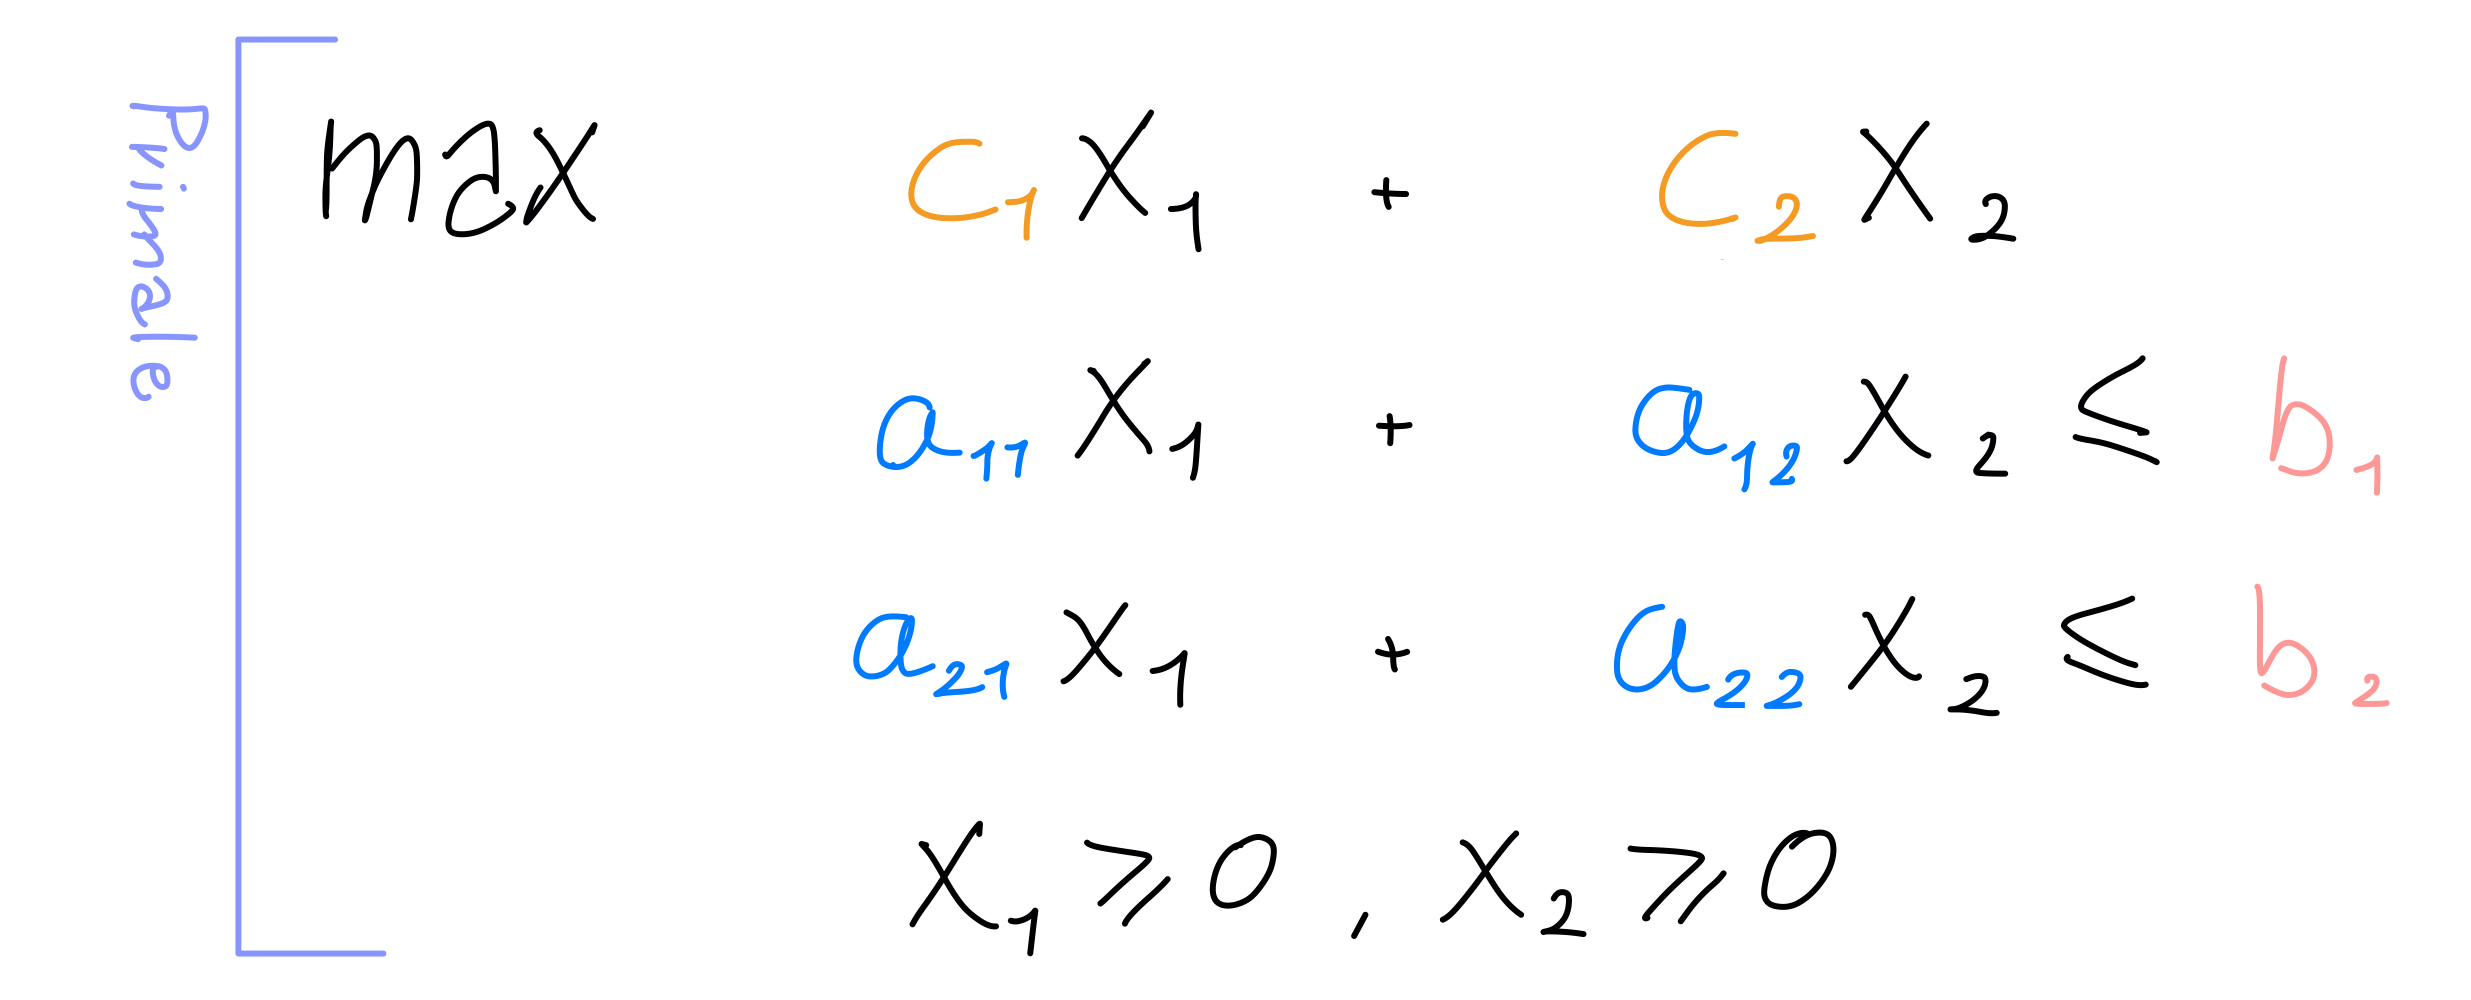
\includegraphics[width=0.8\textwidth]{dualita-cheatsheet-0.jpeg}\\
si riconoscono opportunamente gli elementi che compongono il duale:\\
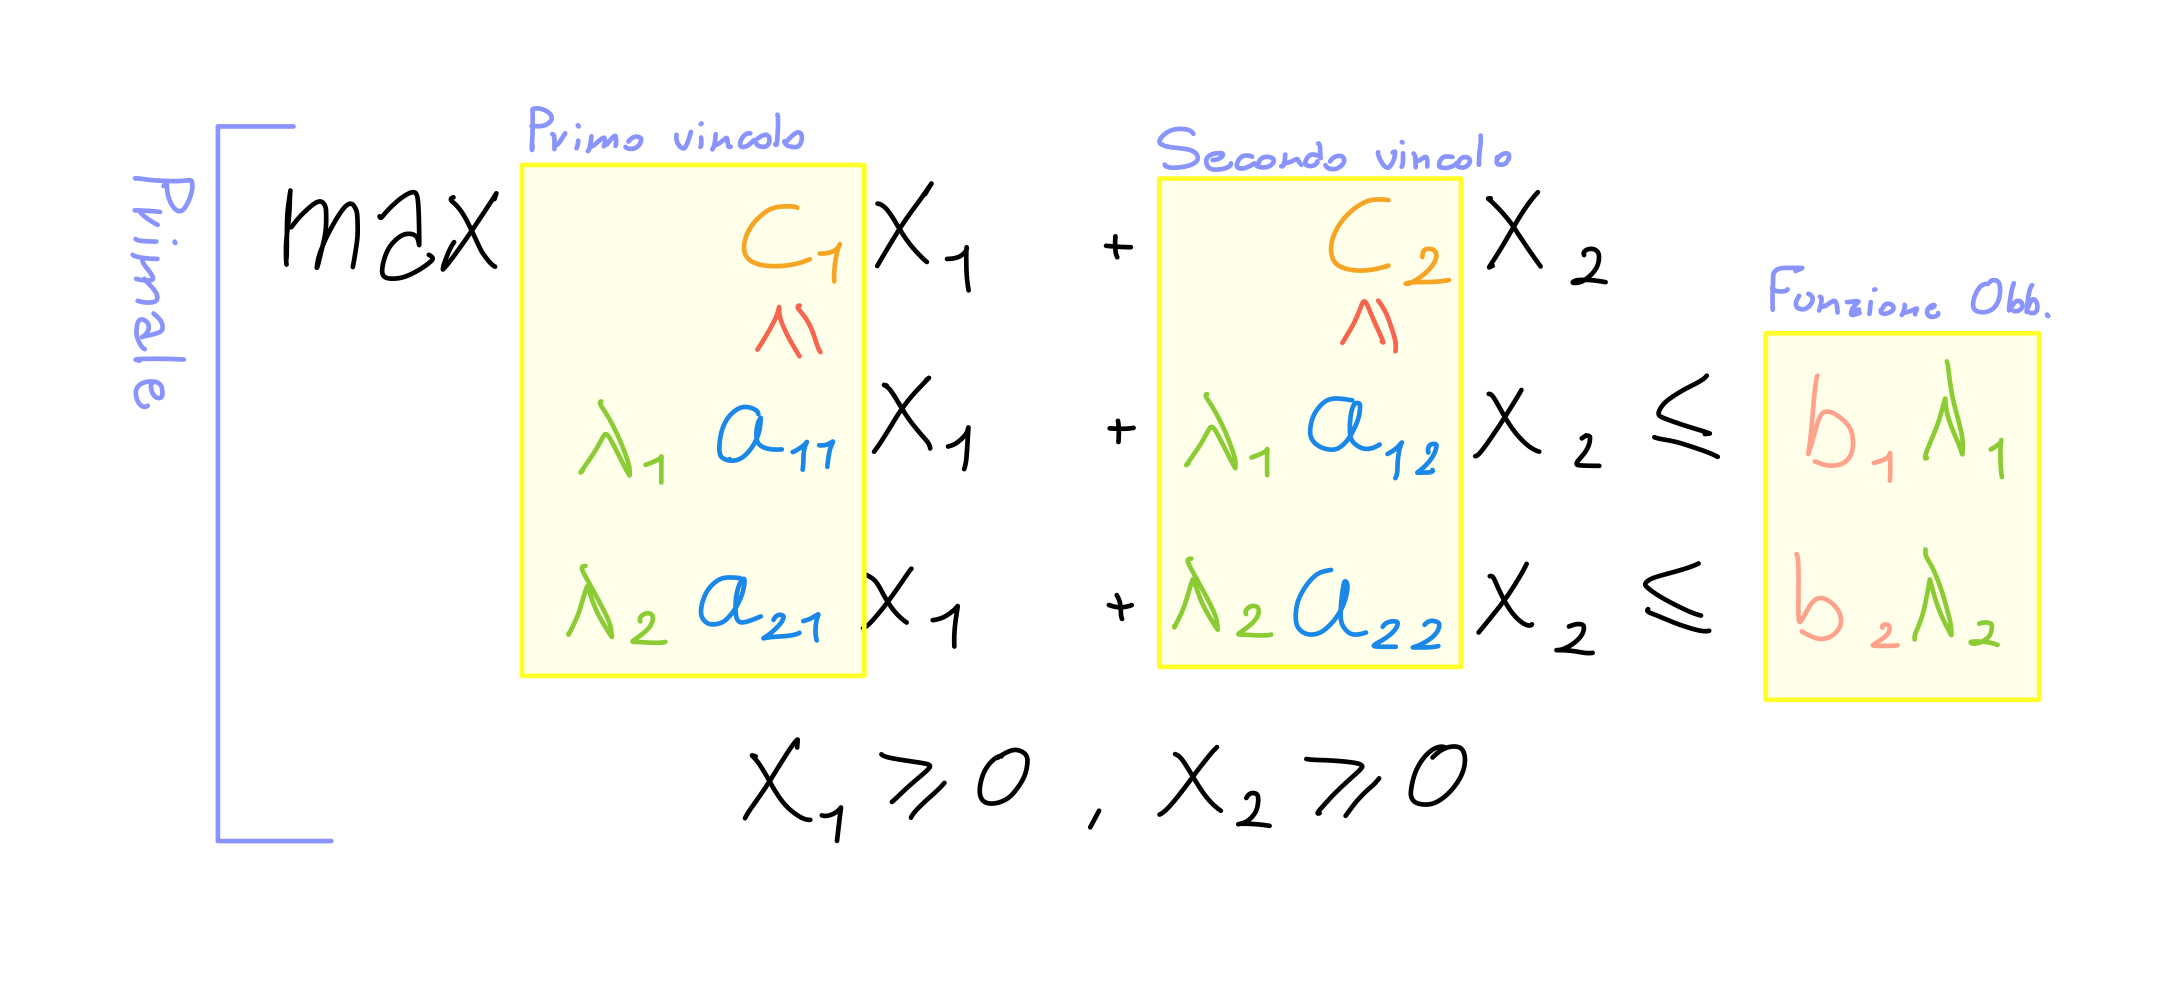
\includegraphics[width=0.8\textwidth]{dualita-cheatsheet-1.jpeg}\\
Che come problema duale generano: \\
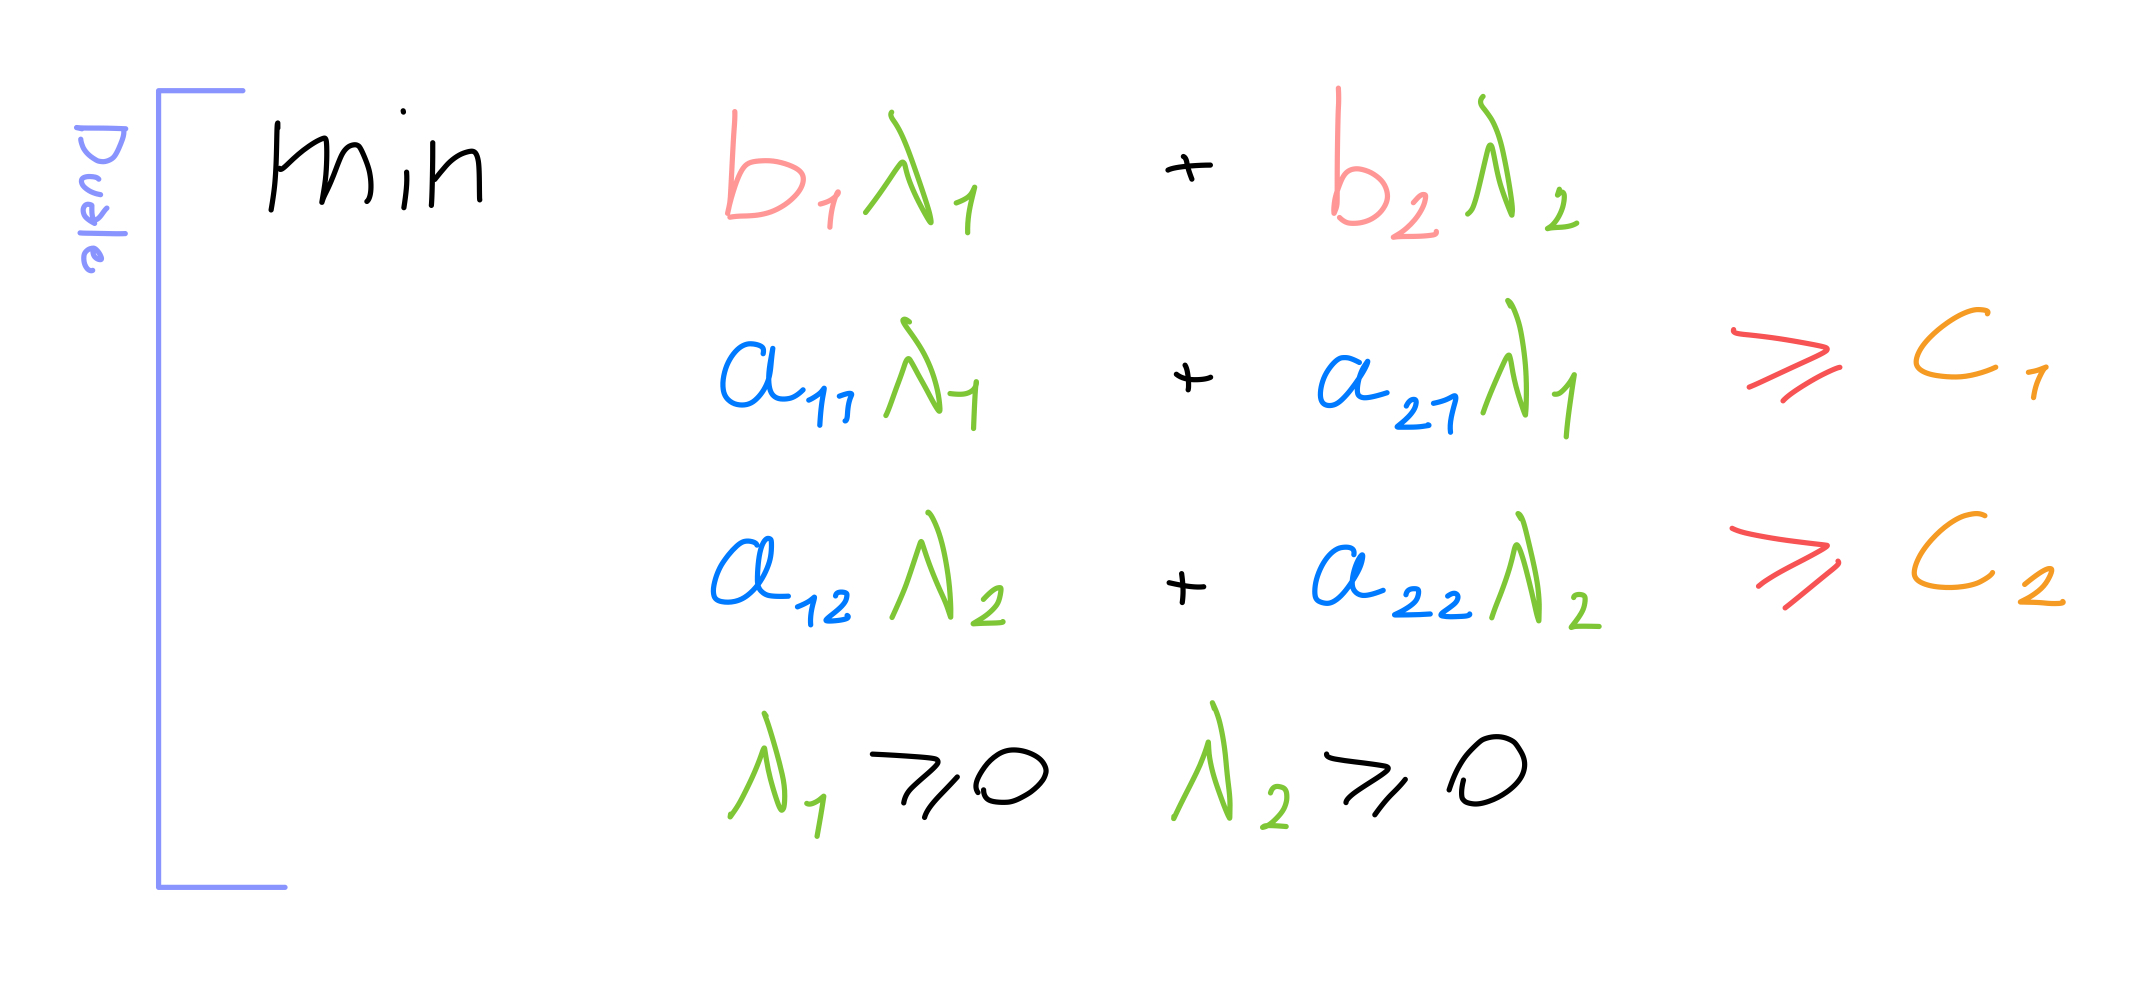
\includegraphics[width=0.8\textwidth]{dualita-cheatsheet-2.jpeg}


\section{Gli Scarti Complementari}
Se abbiamo una soluzione ammissibile per il primale possiamo verificarne l'ottimalità tramite le condizioni degli scarti complementari:
Quindi, data $x^*$:
\begin{tabular}{|c|c|}                                                            
\hline
$x_i^* \neq 0$ & i-esimo (corrispondente) vincolo del duale attivo. \\
\hline
i-esimo vincolo del primale NON attivo & $\lambda_i = 0$\\
\hline
\end{tabular}
Pongo quindi a sistema le equazioni trovate per trovare la soluzione corrispondente del Duale.
Se i valori delle funzioni obiettivo sono uguali, allora le due soluzioni sono entrambe ottime.
	
\chapter{Ottimizzazione Non Lineare}
\section{Algoritmo del Gradiente}
Data una funzione a piú variabili $f(X)$ e un punto $x^0$, ogni passo del metodo del gradiente si effettua in questo modo:

\begin{enumerate}
	\item Calcolo $d^k=\pm \nabla f(x^k)$ ($+$ max e - min)
	\item Calcolo $x^{k+1} = x^k \pm \alpha^k \cdot d^k$
	\item Calcolo $\alpha^k$ come \emph{Max} $f(x^k \pm \alpha^k \cdot d^k)$.
			\\\small{ovvero valuto $f$ nel nuovo punto e massimizzo la funzione risultante $g(\alpha)$, generalmente in modo analitico ($g'(\alpha)=0$)}
	\item Sostituisco $\alpha$ trovato in $x^{k+1}$.
	\item Valuto i criteri di arresto
\end{enumerate}
Per verificare che il punto trovato sia un punto di ottimo, semplicemente controllo che $\nabla f(x^*) = 0$.
\begin{center}
	\begin{tabular}{|l|c|c|}
		\hline
		Nuovo punto & $x^{k+1}$ & $ x^k \pm \alpha^k \cdot d^k$\\
		\hline
		Direzione di Crescita & $d^k$ & $\pm \nabla f(x^k)$ ($+$ max e $-$ min)\\
		\hline
		Step Size & $\alpha^k$ & max $f(x^k \pm \alpha^k \cdot d^k)$\\
		\hline
	\end{tabular}
\end{center}

\pagebreak

\section{Algoritmo di Newton (Multivariato)}
Data una funzione a piú variabili $f(X)$ e un punto $x^0$, una iterazione del metodo di Newton si effettua in questo modo:
\begin{enumerate}
	\item Calcolo $\nabla f(x^k)$ e $H(x^k)$.
	\item Calcolo $V$ Vettore Spostamento: $H_f(x^k) V = - \nabla f(x^k)$
		\\ \small{è un sistema di equazioni, risolvo per $v_1,...,v_n$}
	\item trovo $x^{k+1} = x^k + V$, in cui $V$ é il vettore spostamento.
\end{enumerate}

\begin{center}
	\begin{tabular}{|l|c|c|}
		\hline
		Vettore Spostamento &$V$& $H_f(x^k) V = - \nabla f(x^k)$\\
		\hline
		Nuovo punto & $x^{k+1}$ & $ x^k + V $\\
		\hline
	\end{tabular}
\end{center}


\chapter{Ottimizzazione Non Lineare Vincolata}
\section{Funzione Lagrangiana}
In un problema di ottimizzazione vincolata definito come:
\begin{center}
	opt $f(x_1,...,x_n)$,
	\\
	$g_m(x_1,...,x_n) = 0$ Vincoli di Uguaglianza,
	\\
	$h_l(x_1,...,x_n) \leq 0$ Vincoli di Disguaglianza,
\end{center}
Generiamo la Lagrangiana cosí definita:
\[
	L(V) = f(X) \pm \sum_{i=0}^{m} \lambda_i \cdot g_i(X) \pm \sum_{j=0}^{l} \mu_j \cdot h_j(X)
\]
in cui $\pm$ diventa $+$ per i problemi di MIN e $-$ per i problemi di MAX,
Abbiamo che $\lambda$ sono i moltiplicatori lagrangiani associati ai vincoli di Uguaglianza, e $\mu$ quelli associati ai vincoli di Disuguaglianza.
\\\small{con $V=\{x_1,...,x_n,\lambda_1,...,\lambda_m, \mu_1,...,\mu_l\}$, ovvero tutte le variabili e $X=\{x_1,...,x_n\}$, ovvero tutte le variabili origniali.}

\section{Condizioni KKT}
\paragraph{Tabella}
Bisogna quindi generare un sistema che avrá $n+m+l$ incognite utilizzando le KKT,
riportate qui in modo semplificato:\\
\begin{tabularx}{\textwidth}{|Y|}
	\hline
	Stazionarietá Problemi di MIN (-)                                             \\
	$ \nabla f = - \sum \lambda_i \cdot \nabla g_i - \sum \mu_j \cdot \nabla h_j$ \\
	\hline \hline
	Stazionarietá Problemi di MAX (+)                                             \\
	$ \nabla f = + \sum \lambda_i \cdot \nabla g_i + \sum \mu_j \cdot \nabla h_j$ \\
	\hline
\end{tabularx}\\
\begin{tabularx}{\textwidth}{|l|cY|}
	\hline
	Ammissibilitá Vincoli Uguaglianza    & $\forall$  & $ g_i = 0$             \\
	\hline
	Ammissibilitá Vincoli Disuguaglianza & $ \forall$ & $ h_j\leq 0$           \\
	\hline
	Condizione di Complementarietá       & $\forall$  & $ \mu_j \cdot h_j = 0$ \\
	\hline
	Non Negativitá di $\mu$              & $\forall $ & $ \mu_j \geq 0$        \\
	\hline
\end{tabularx}
\\Dove con $\forall$ si intende chiaramente tutti quelli presenti.


\subsection{Differenziare tra Max e Min}
Quando si usano le KKT bisogna differenziare tra problemi di Max e Problemi di Min.
Ogni problema ha le seguenti possibili combinazioni:\\
\begin{tabularx}{\textwidth}{|l|c|Y|}
	\hline
	\multirow{2}{*}{\textbf{Problema di Massimo}} & \textcolor{gray}{ $\mu_i\geq 0$ }& \textcolor{gray}{ $ \nabla f = + \sum \lambda_i \cdot \nabla g_i + \sum \mu_j \cdot \nabla h_j$} \\
	\cline{2-3}& \textcolor{black}{$\mu_i\leq 0$} & \multirow{2}{*}{\textcolor{black}{$ \nabla f = - \sum \lambda_i \cdot \nabla g_i - \sum \mu_j \cdot \nabla h_j$}} \\
	\cline{1-2}
	\multirow{2}{*}{\textbf{Problema di Minimo}} &\textcolor{black}{$\mu_i\geq 0$} & \\
	\cline{2-3}&\textcolor{gray}{ $\mu_i\leq 0$} & \textcolor{gray}{$ \nabla f = + \sum \lambda_i \cdot \nabla g_i + \sum \mu_j \cdot \nabla h_j$} \\
	\hline
\end{tabularx}
é utile sapere che se scegliessimo di avere la funzione obiettivo \textbf{Sempre come somma di elementi negativi}, sia per i problemi di massimo che di minimo,
allora potremmo, in base ai valori di $\mu$, sapere in un solo calcolo se il punto é candidato a massimo o minimo.

\subsection{Risolvere il Sistema}
Per risolvere il sistema, o lo si risolve con il metodo classico, oppure tramite questo metodo:
Con la condizione di \textbf{Complementarietá} sappiamo che: \[\mu_j \cdot h_j = 0 \implies \mu_j = 0 \vee h_j = 0\]
Quindi, con $l$ variabili $mu_j$ abbiamo $2^l$ combinazioni di sistemi, in cui $mu_j = 0 \vee \mu_j \neq 0$.
Cosí possiamo risolvere le $2^l$ combinazioni per trovare tutti i punti candidati. 

\subsection{Trovare i punti di Minimo e Massimo}
I punti trovati dalle condizioni KKT sono solo candidati a essere punti di max/min, perché le KKT sono condizioni Necessarie ma non Sufficienti.

Le condizioni KKT diventano Sufficienti se:
\begin{itemize}
	\item Per i Punti di Massimo:
	 \begin{itemize}
		\item $f$ é concava.
		\item I vincoli $h_i(X)$ sono tutti Convessi.
	\end{itemize}
	\item Per i Punti di Minimo:
	\begin{itemize}
	   \item $f$ é convessa.
	   \item I vincoli $h_i(X)$ sono tutti Convessi.
   \end{itemize}
\end{itemize}

\end{document}